\chapter{Structural Results}\label{chap:structural-results}


This chapter shall be devoted to looking at some structural results on arithmetic circuits. This would help us understand the relevance of shallow circuits in the context of proving lower bounds for arithmetic circuits of arbitrary depth. 

\section{Homogenization}\label{sec:homogenization}

Suppose we have an $n$-variate degree $d$ polynomial computed by an arithmetic circuit $C$. How large can the degree of intermediate computations be? Potentially, intermediate computations can involve very high degree terms which somehow cancel each other at the root. However, the following lemma of Strassen shows that we may assume without much loss of generality that arithmetic circuits never compute polynomials of degree more than the output. 

\begin{definition}[Homogeneous circuits]
A circuit $C$ is said to be \emph{homogeneous} if every gate in the circuit computes a homogeneous polynomial. 
\end{definition}

\begin{lemma}[Homogenization]\label{lem:homogenization}
Let $f$ be an $n$-variate degree $d$ polynomial computed by a circuit $C$ of size $s$. Then, for every $0\leq i \leq d$, there is a \emph{homogeneous arithmetic circuit} $C_i'$, of size at most $O(sd^2)$, that computes the degree $i$ homogeneous polynomial in $i$. 
\end{lemma}
\begin{proof}
Assume without loss of generality that the circuit $C$ has all gates with fan-in at most $2$. 
For every gate $g\in C$, define $(d+1)$ gates $g^{(0)},\dots, g^{(d)}$; we shall construct a new circuit $C'$ such that $g^{(i)}$ computes the degree $i$ homogeneous part of the polynomial computed at $g$. If $g$ has children $h_1$ and $h_2$, then $C'$ would have the following connections depending on the type of the gate $g$:
\begin{eqnarray*}
\text{$g = h_1 + h_2$}\quad\implies\quad g^{(i)} &=& h_1^{(i)} \spaced{+} h_2^{(i)}\quad\text{for all $i$}\\
\text{$g = h_1 \times h_2$}\quad\implies\quad g^{(i)} &=& \sum_{j=0}^i h_1^{(j)} h_2^{(i-j)}\quad\text{for all $i$}
\end{eqnarray*}
It is easy to check that the size of the circuit $C'$ is at most $O(sd^2)$, and computes all the homogeneous components of $f$. 
\end{proof}

Thus, for arithmetic circuits, we can assume without much loss of generality that we are working with a homogeneous circuit. 

\begin{remark*}
For the class of arithmetic formulas, it is not clear if we can homogeneous without loss of generality. If we were to apply the above lemma to an arbitrary arithmetic formula, the resulting object is a homogeneous circuit and not a formula. It is unclear if any formula can be homogenized without loss of generality. The same is the case even for constant depth circuits, as the above construction does not preserve the depth of the circuit. 

However, the class of ABPs can also be assumed to be homogeneous without loss of generality. We leave this as an exercise. 
\end{remark*}

\begin{exercise}
Prove a similar homogenization lemma for arithmetic branching programs. 
\end{exercise}

\section{Depth reduction}

The phenomenon of simulating an arbitrary arithmetic circuit by a \emph{shallow} arithmetic circuit is called \emph{depth reduction}. Arithmetic circuits exhibit some remarkable depth reduction results, and we shall go over these in this section. 

\subsection{Depth reduction for arithmetic formulas}

The depth reduction for formulas is quite easy to describe. This would also serve as step towards understanding the depth reduction for arithmetic circuits. The following depth reduction is due to Brent~\cite{brent74}. 

\begin{lemma}[\cite{brent74}]\label{lem:formula-depth-reduction}
Let $f$ be an $n$-variate degree $d$ polynomial computed by an arithmetic formula $\Phi$ of size $s$. Then, $f$ can also be computed by a formula $\Phi'$ of size $s' = \poly(s,n,d)$ and depth $O(\log s)$. 
\end{lemma}
\begin{proof}
Assume without loss of generality that $\Phi$ is a formula of fan-in $2$. Starting from the root, walk down to the leaves by always taking the child with a larger sub-tree under it. Consider the first node in this path $v$ such that the size of the formula rooted at $v$ is smaller than $\frac{2s}{3}$. Let $\Phi_v$ refer to the sub-formula rooted at $v$. By the choice of the path from the root, we have
\[
\frac{s}{3} \spaced{\leq} \abs{\Phi_v} \spaced{<} \frac{2s}{3}.
\]
Let $\hat{\Phi}_v$ denote the formula where the sub-formula at $v$ is replaced by a fresh variable $y$. Since we are dealing with formulas, $\hat{\Phi}_v$ is a linear polynomial in the variable $y$. Hence,
\begin{eqnarray*}
\hat{\Phi}_v(y) & = & A \cdot y \spaced{+} B\\
\text{and,}\quad \Phi & = & A \cdot \Phi_v \spaced{+} B
\end{eqnarray*}
for some polynomials $A$ and $B$. But we can compute both $A$ and $B$ from $\hat{\Phi}_v(y)$ as
\begin{eqnarray*}
A & = & \hat{\Phi}_v(1) - \hat{\Phi}_v(0)\\
B & = & \hat{\Phi}_v(0)
\end{eqnarray*}
Thus, 
\[
f \quad = \quad (\hat{\Phi}_v(1) - \hat{\Phi}_v(0))\cdot \Phi_v \spaced{+} \hat{\Phi}_v(0)
\]
All the formulas in the above equation have size at most $\frac{2s}{3}$. Thus, by recursively applying this process on each of these sub-formulas, we obtain an $O(\log s)$ depth formula of size $\poly(s)$ as claimed. 
\end{proof}

\begin{figure}
\begin{center}
\tikzstyle{gate}=[circle,draw=black!50,thick]
\tikzstyle{leaf}=[circle,draw=black!50,fill=black!10,thick]
\tikzstyle{phi}=[rectangle,draw=black!50,fill=black!10,thick]
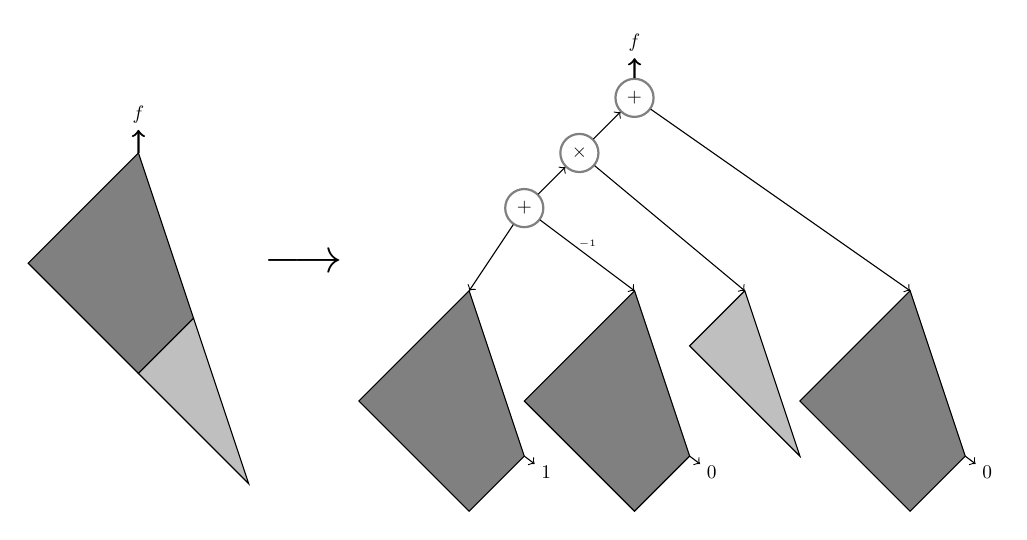
\begin{tikzpicture}[transform shape, scale=0.7]
  \draw[fill=gray] (-10,-2) -- ++(-2,-2) -- ++(2,-2) -- ++(1,1) -- cycle;
  \draw[fill=gray!50] (-9,-5) -- ++(1,-3) -- ++(-2,2) -- cycle;

    \node at (-10,-1.3) {$f$}
    edge[<-,thick] (-10,-2) ;

  
  \node at (-7,-4) {\Huge $\longrightarrow$};
  
  \node (ph) at (-1,0) {$f$};
  \node[gate] (root) at (-1,-1) {$+$}
  edge[thick,->] (ph)
  edge[->] (4,-4.5);
  \node[gate] (m1) at (-2,-2) {$\times$}
  edge[->] (root)
  edge[->] (1,-4.5);
  
  \draw[fill=gray] (4,-4.5) -- ++(-2,-2) -- ++(2,-2) -- ++(1,1) -- cycle;
  \node at  (5.4,-7.8) { $0$}
  edge[<-] (5,-7.5);
  
  \node[gate] (s1) at (-3,-3) {$+$}
  edge[->] (m1)
  edge[->] (-4,-4.5)
  edge[->] node[above] {\tiny $-1$} (-1,-4.5);
  
  \draw[fill=gray!50] (1,-4.5) -- ++(1,-3) -- ++(-2,2) -- cycle;
  
  
  \draw[fill=gray] (-4,-4.5) -- ++(-2,-2) -- ++(2,-2) -- ++(1,1) -- cycle;
  \node at  (-2.6,-7.8) { $1$}
  edge[<-] (-3,-7.5);
  
  \draw[fill=gray] (-1,-4.5) -- ++(-2,-2) -- ++(2,-2) -- ++(1,1) -- cycle;
  \node at  (0.4,-7.8) { $0$}
  edge[<-] (0,-7.5);
\end{tikzpicture}
\end{center}
\caption{Depth reduction for formulas}
\label{fig:formula-depth-red}
\end{figure}

\subsection{Depth reduction for arithmetic circuits}

The key point in the above depth reduction was that for any node $v$, the formulas $\Phi_v$ and $\hat{\Phi}_v(y)$ were disjoint. This however is not the case for general arithmetic circuits. Thus, it is not clear if we can find a node in the circuit such that the subcircuit under it has size between $s/3$ and $2s/3$. However, we do not really need to make the subcircuits have size drop by a constant factor, but any parameter dropping by a constant factor would be okay. One parameter that we could work with instead is the \emph{degree}. Valiant, Skyum, Berkowitz and Rackoff \cite{vsbr83} showed that one could achieve a similar depth reduction for general circuits. This section shall be devoted to the proof of their remarkable theorem.\footnote{The proof described here follows the structure of a subsequent result \cite{ajmv98}, and not the original proof, although both proofs are quite similar.}

\begin{theorem}[\cite{vsbr83}]\label{thm:vsbr}
Let $f$ be an $n$-variate degree $d$ polynomial computed by an arithmetic circuit $\Phi$ of size $s$. Then, there is an arithmetic circuit $\Phi'$ computing $f$ and has size $s' = \poly(s,n,d)$ and depth $O(\log d)$. 
\end{theorem}

By Lemma~\ref{lem:homogenization}, we may assume without loss of generality that $\Phi$ is a homogeneous circuit. We will also assume that in $\Phi$, all multiplication gates have fan-in at most $2$ (this might increase the depth of $\Phi$ by a factor of $\log s$, but this would not hurt us). Now, we can find a similar ``$\inparen{\frac{1}{3},\frac{2}{3}}$ separator'' as in the proof of Lemma~\ref{lem:formula-depth-reduction}, but based on degree instead of size. 

\begin{claim}
Let $\Phi$ be a homogeneous arithmetic circuit computing a homogeneous degree $d$ polynomial, where each multiplication gate has fan-in at most $2$. Then, there exists a node $v$ that computes a polynomial of degree $d'$ satisfying $d/3 \leq d' \leq 2d/3$. 
\end{claim}

The proof is exactly the same, except now you take a path from root to leaf by always going through the child of larger degree. What can we say about replacing the entire sub-circuit at $v$ by a new variable $y$? This runs in to some immediate problems. What if there was a node $w$ in the subcircuit at $v$, which is maybe connected to other nodes in $\Phi$? Also, the polynomial $\hat{\Phi}_v(y)$ could continue to have degree as large as $d$. Thus it is not clear if this approach would help us make progress. 

The cause of all these problems stems because the node $v$ could reached from the root through multiple paths, and hence needs to be treated with care. However, with a little more care, we can still mimic the earlier depth reduction for formulas. \\

Let us go over every gate in $\Phi$, and reorder the children so that the children are sorted in decreasing order of degrees (with the left child being the one with largest degree). We shall call such circuits as \emph{left-heavy} circuits. Note that the proof of the claim above yields such a node $v$ on the left-most path of $\Phi$. 

Since any polynomial is a sum of monomials, it would be useful to break the computation by an arbitrary circuits by a sum of smaller computations each corresponding to a monomial. The following definition does just that. 

\begin{definition}[Proof trees]\label{defn:proof-tree}
A \emph{proof tree} of an arithmetic circuit $C$ is a sub-graph $T$ obtained as follows:
\begin{itemize}
\item The root of $C$ is in $T$.
\item For every addition gate $g\in T$, the subgraph $T$ also contains \emph{exactly one} of its children.
\item For every multiplication gate $g\in T$, the subgraph $T$ also contains \emph{both} its children. 
\end{itemize}
\end{definition}

A proof tree naturally computes a single monomial, and is a minimal witness that a certain monomial is computed in by the circuit. (It is however possible that the same monomial can be computed by multiple proof trees and there could be several cancellations.)

A very natural question at this point is why is a \emph{proof tree} a tree! It isn't clear from the above definition but note that all proof trees of a homogeneous circuit $C$ (computing a degree $d$ polynomial) computes a monomial of degree $d$. Thus, the number of multiplication gates in any proof tree is at most $d$. Thus, we may unravel any proof tree $T$ to an actual tree $T$ while not increasing the size by much. Thus, without loss of generality, we may assume that all proof trees of $C$ are unravelled to indeed be trees. 

We shall denote the set of all proof trees of a circuit $C$ by $\mathrm{ProofTrees}(C)$. Also, for any node $u\in C$, we shall use $\mathrm{ProofTree}(u)$ to refer to the set of all proof trees rooted at $u$. Further, for any proof tree $T$, we shall use $\mathrm{eval}(T)$ to denote  the  \emph{monomial computed by $T$}. Thus, if $f$ is the polynomial computed by a circuit $C$, then
\[
f\spaced{=} \sum_{T\in \mathrm{ProofTrees}(C)} \mathrm{eval}(T)
\]

With this definition, we can now apply a Brent-like argument on \emph{proof trees} rather than the actual circuit itself. Recall that in the proof of Lemma~\ref{lem:formula-depth-reduction}, we expressed $\Phi$ as a linear function of $A \Phi_v + B$. The following notation captures the quotient $A$, but now in the case of general circuits via the notation of proof trees. 

\begin{definition}[Proof tree quotients]
For any proof tree $T$, and a node $v$, define the operation $\mathrm{snip}_v(T)$ as
\begin{itemize}
  \item If $v$ does not appear in the left-most path of $T$, then $\mathrm{snip}_v(T) = 0$
  \item If $v$ does appear in the left-most path of $T$, then $\mathrm{snip}_v(T)$ refers to the tree obtained by replacing the node $v$ on the left-most path by a leaf labelled $1$. 
\end{itemize}
For any two nodes $u$ and $v$ in the circuit $C$, the polynomial $[u:v]$ is defined as
\[
[u:v] \spaced{=} \sum_{T \in \mathrm{ProofTrees}(u)} \mathrm{eval}(\mathrm{snip}_v(T))
\]
\end{definition}

Intuitively, $[u:v]$ refers to the \emph{suffix} of $v$ in the computation at $u$. By only snipping off $v$ from the left-most path, this allows us to get a better control with the issue of $v$ occurring multiple times in the proof tree. For a formula $\Phi$, the polynomial $[\Phi:v]$ would refer to $\hat{\Phi}_v(1)$. Note that $[u:v]$ is a polynomial of degree $\deg(u) - \deg(v)$. \\

The next thing we would like to do using the above notation is to rewrite the polynomial computed at $u$ by a sum involving several $[u:v_i]$s for suitable choice of $v_i$. To do this, we need to identify a set of nodes $\inbrace{v_i}$ such that the left-most path of every proof tree $T$ passes through exactly one $v_i$ from this set. One example of such a set is just the set of leaves. Thus, we can express the polynomial computed at any node $u$ as
\[
[u] \spaced{=} \sum_{i} [u:x_i] \cdot x_i
\]
In fact, a more general construction could be defined for any parameter $t$ as
\[
\mathcal{F}_t  \spaced{=} \setdef{w\in C}{\deg(w) \geq t \spaced{\&} \deg(w_L) < t}
\]
where $w_L$ refers to the left child of $w$. When we have nodes $u,v \in C$, we shall use $\mathrm{Frontier}(u)$ to refer to $\mathcal{F}_t$ where $t = \deg(u)/2$ and $\mathrm{Frontier}(u:v)$ to refer to $\mathcal{F}_t$ for $t = \deg(u:v)/2$. It is worth noting that all nodes in $\mathcal{F}_t$ must be multiplication gates (since the children have strictly smaller degree). 


\begin{observation}
The left-most path of any proof tree $T$ of $u$ passes through exactly one node in $\mathrm{Frontier}(u)$. The same applies to $\mathrm{Frontier}(u:v)$ as well. 
\end{observation}

With this observation, we have the sums we were looking for. 

\begin{eqnarray}\label{eqn:VSBR-split-frontier}
\text{For any $u\in C$,}\quad\quad [u] &=& \sum_{v\in \mathrm{Frontier}(u)} [u:v]\cdot [v] \label{eqn:VSBR-split-frontier-u}\\
\text{For any $u,v\in C$,}\quad\quad [u:v] &=& \sum_{w\in \mathrm{Frontier}(u:v)} [u:w]\cdot [w:v] \label{eqn:VSBR-split-frontier-u:v}
\end{eqnarray}

With these in hand, we can now describe the depth-reduced circuit of \cite{vsbr83}. 

For each $u \in C$, the circuit $C'$ has a node computing $[u]$, and for every pair of nodes $u,v\in C$, there is a node in $C'$ computing $[u:v]$. To describe how $[u]$ is computed in $C'$, start with equation \eqref{eqn:VSBR-split-frontier-u}
\begin{eqnarray*}
[u] &=& \sum_{v\in \mathrm{Frontier}(u)} [u:v]\cdot [v]\\
 & = & \sum_{v\in \mathrm{Frontier}(u)} [u:v] \cdot [v_L] \cdot [v_R]
\end{eqnarray*}
Note that since $v\in \mathrm{Frontier}(u)$, we have that $\deg(v) \geq \deg(u)/2$ and $\deg(v_R),\deg(v_L) < \deg(u)/2$. Thus each of the three terms in every summand of the above equation has degree at most half the degree $u$. The computation of $[u:v]$'s are a little more involved. By equation \eqref{eqn:VSBR-split-frontier-u:v}, we have
\begin{eqnarray*}
[u:v] &=& \sum_{w\in \mathrm{Frontier}(u:v)} [u:w]\cdot [w:v]\\
      &=& \sum_{w\in \mathrm{Frontier}(u:v)} [u:w]\cdot [w_R]\cdot  [w_L:v]
\end{eqnarray*}
Since every $w \in \mathrm{Frontier}(u:v)$, we have that $\deg(u:w),\deg(w_L:v) \leq \deg(u:v)/2$. The issue is that $[w_R]$ could have pretty large degree. To see this, note that $w$ is a node of degree between $\deg(u)$ and $\deg(v)$. Thus, it is possible that $(u:w)$ and $(w_L:v)$ have very small degree and $\deg(w_R)$ could be as large as $\deg(u:v)$. However, we can expand $[w_R]$ using \eqref{eqn:VSBR-split-frontier-u} and we would then have what we want. 
\begin{eqnarray*}
[u:v] &=& \sum_{w\in \mathrm{Frontier}(u:v)} [u:w]\cdot [w_R]\cdot  [w_L:v]\\
      &=& \sum_{w\in \mathrm{Frontier}(u:v)} [u:w]\cdot \inparen{\sum_{p \in \mathrm{Frontier}(w_L)} [w_R:p] \cdot [p_L] \cdot [p_R]} \cdot  [w_L:v]
\end{eqnarray*}
Observe that we have $\deg (u:w), \deg(w_L:v) \leq \deg(u:v)/2$ from earlier, and we also have
\begin{eqnarray*}
\deg(u:w),\deg(w_L:v) & \leq &\frac{\deg(u:v)}{2}\\
\deg(w_R:p),\deg(p_L),\deg(p_R) & \leq & \frac{\deg(w_R)}{2}\\
 & \leq & \frac{\deg(u:v)}{2}
\end{eqnarray*}
Thus, once again, we are in the situation where all the factors in the RHS have at most half the degree of the RHS. Thus, this shows that every $(u:v)$ can be computed by an arithmetic circuit $C'$ of size $\poly(s)$ and depth $O(\log d)$. In particular, $f = [\mathrm{root}]$ can be computed be computed by $C'$, as claimed. \qed {(\footnotesize Theorem~\ref{thm:vsbr})}\\

\begin{remark}\label{remark:vsbr}
From the proof above, we can see that the resulting circuit $C'$ has useful structural properties. 
\begin{itemize}
  \item The circuit is homogeneous. 
  \item Addition gates have fan-in bounded by $\poly(s)$. 
  \item Multiplication gates have fan-in bounded by $5$. 
  \item If $u$ is any multiplication gate, then all its children $v$ satisfy $\deg([v])\leq \deg([u])/2$. 
\end{itemize}
\end{remark}

These additional properties would be useful in the next section, where we shall squash $C'$ down to a depth four circuit!

\subsection{Reduction to depth four circuits}

One of the consequence of a depth reduction such as Theorem~\ref{thm:vsbr} is that proving lower bounds for general circuits is reduced to the task of proving lower bounds for $O(\log d)$ depth circuits. 

\begin{corollary}\label{cor:vsbr-contra}
If $f$ is an $n$-variate degree $d$ polynomial that requires super-polynomial (in $n$ and $d$) size circuits of $O(\log d)$ depth to compute it, then any general arithmetic circuit computing $f$ must also be of super-polynomial size. 
\end{corollary}

But, optimistically, we would expect that the \emph{right} lower bound must be truly exponential, and not merely super-polynomial. Keeping that in mind, a depth reduction even with a slightly super-polynomial blow-up might be useful in this regard. This line was first pursued by Agrawal and Vinay \cite{av08}, and the result was subsequently strengthened by Koiran \cite{koiran} and Tavenas~\cite{Tav13}. 

\begin{theorem}[\cite{av08,koiran,Tav13}] \label{thm:av}
Let $f$ be an $n$-variate degree $d$ polynomial computed by a size $s$ arithmetic circuit. Then for any $0< t \leq d$, $f$ can be equivalently computed by a homogeneous $\SPSP^{[t]}$ circuit of top fan-in $s^{O(d/t)}$ and size $s^{O(t + d/t)}$. 
\end{theorem}

If we were to optimize the size of the final depth four circuit, then we should choose $t = \sqrt{d}$ to get a $\SPSP^{[t]}$ circuit of size $s^{O(\sqrt{d})}$. Note that this implies that if we could prove a lower bound of $n^{\omega(\sqrt{d})}$ for such $\SPSP^{[\sqrt{d}]}$ circuits, then we would have proved a lower bound for general circuits! In fact, in the recent past, we have come pretty close to the required threshold and we shall see them in the later chapters. \\

In this section, we shall see a proof of Theorem~\ref{thm:av} but this is not the original proof of Tavenas~\cite{Tav13}. We shall see an alternate proof by \cite{saptharishivinay14}, which I find more insightful. 

\begin{proofof}{Theorem~\ref{thm:av}}
Let $C$ be the $O(\log d)$ depth  circuit computing $f$ obtained from Theorem~\ref{thm:vsbr} applied on the size $s$ circuit computing $f$. Let $s'$ be the size of $C$. If $g$ is a polynomial computed at any intermediate node of $C$, then from the structure of $C$ (Remark~\ref{remark:vsbr}) we have a homogeneous expression
\begin{equation}\label{eqn:vsbr-expansion}
g \spaced{=} \sum_{i=1}^{s'} g_{i1} \cdot g_{i2} \cdot g_{i3} \cdot g_{i4} \cdot g_{i5} 
\end{equation}
where each $g_{ij}$ is computed by a node in $C$ as well, and $\deg(g_{ij}) \leq \deg(g)/2$. If we look at \eqref{eqn:vsbr-expansion} for $f$, then the RHS is a $\SPSP^{[d/2]}$ circuit of top fan-in $s'$ computing $f$. To obtain a $\SPSP^{[t]}$ circuit eventually, we shall do the following natural process. 
\begin{quote}
  For each summand $g_{i1}\dots g_{ir}$ in the RHS, if the largest degree $g_{ij}$ has degree more than $t$, expand that $g_{ij}$ in-place using \eqref{eqn:vsbr-expansion}. 
  
  Repeat this process until all $g_{ij}$'s on the RHS have degree at most $t$. 
\end{quote}

Note that in each iteration of the above procedure, we increase the top fan-in by a multiplicative factor of $s'$, and what we gain is that some the terms in the RHS would now have smaller degrees. If we could show that the in $O(d/t)$  iterations  all terms on the RHS have degree at most $t$, then we would have obtained an $\SPSP^{[t]}$ circuit of top fanin $s'^{O(d/t)}$ computing $f$. \\

To bound the number of iterations, let us count the number of terms of degree more than $t/8$ in each term. Note that since we would always maintain homogeneity, the number of terms of degree  $t/8$ or more in any summand  is at most $8d/t$. Thus, it suffices to show that each iteration increases the number of terms of degree $t/8$ by at least one. 

Note that in \eqref{eqn:vsbr-expansion}, if $\deg(g) = d'$ then the largest degree term of any summand on the RHS is at least $d'/5$ (since the sum of the degrees of the five terms must add up to $d'$). Also, the largest degree term can have degree at most $d'/2$. Hence there must be at least $d'/2$ degree contributed by the other four factors in each term. This implies that the second largest factor in each summand has degree at least $d'/8$. Therefore, as long as we are expanding factors using \eqref{eqn:vsbr-expansion} of degree more than $t/8$, we are guaranteed that each new term has at least one more factor of degree more than $t/8$. As argued earlier, we can never have more than $8d/t$ such terms in any summand and this bounds the number of iterations by $8d/t$. 

Thus, when the above procedure stops, we have an $\SPSP^{[t]}$ circuit of top fan-in $s'^{O(8d/t)} = s^{O(d/t)}$. Observing that any polynomial of degree $t$ can have at most $n^t$ monomials, we get that the size of the circuit overall is at most $s^{O(t + d/t)}$. 
\end{proofof}

Thus, proving a ``good enough'' top fanin (or size) lower bound for the class of $\SPSP^{[t]}$ circuit would suffice for proving lower bounds for general circuits. We would be using this fact quite a lot so we state this explicitly as a corollary. 

\begin{corollary}\label{cor:av}
If $f$ is an $n$-variate degree $d$ polynomial that requires homogeneous $\SPSP^{[t]}$ circuits of top fan-in $n^{\omega(d/t)}$ to compute it, then $f$ requires general arithmetic circuits of size $n^{\omega(1)}$ to compute it. 
\end{corollary}

\subsection*{Further depth reductions}

There have been some further depth reductions results, but we shall defer that to later in the interest of presenting more insight and intuition. They would be better placed after we have seen a few of the recent lower bounds for restricted depth four circuits. We now proceed to see some lower bounds. 



%%% Local Variables: 
%%% mode: latex
%%% TeX-master: "main"
%%% End: 